\scanpage{48}
\mspage{\handwritten{16}}
\uline{Alors, pour tout sous-$\handwritten{\mathcal{O}}_S$-Module quasi-cohérent $\handwritten{\mathcal{F}}$ de $\handwritten{\mathcal{E}}$ il existe un plus petit sous-$\handwritten{\mathcal{O}}_S$-Module quasi-cohérent $\handwritten{\widetilde{\mathcal{F}}}$ de $\handwritten{\mathcal{E}}$ contenant $\handwritten{\mathcal{F}}$ qui soit stable sous $\handwritten{\rho}$.}\inserted{\figure{\handwritten{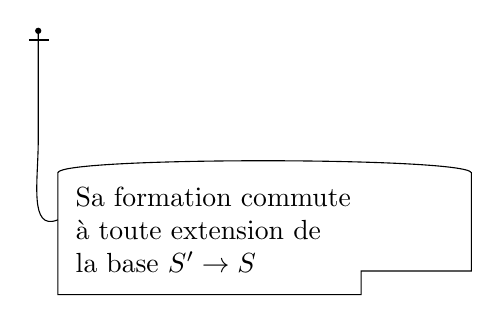
\begin{tikzpicture}[x=1cm,y=1cm]
\draw (.25,.1) .. controls (-.12,-.05) and (0,.6) .. (0,1.1) -- (0,2.5);
\fill (0,2.5) circle (.04);\draw[line width=.8pt] (-.12,2.38) -- (.14,2.38);
\draw (.25,.7) .. controls (.3,.9) and (5.4,.9) .. (5.5,.7) -- (5.5,-.55) -- (4.1,-.55) -- (4.1,-.85) -- (.25,-.85) -- cycle;
\node[align=left,anchor=west] at (.35,-.03) {Sa formation commute\\à toute extension de\\la base $S'\to S$};
\end{tikzpicture}}}}\uline{Lorsque $\handwritten{\mathcal{F}}$ est de type \deleted{\illegible{1}} fini, il en est de même de $\handwritten{\mathcal{F}}$.}

On se ramène aisément\inserted{\handwritten{par descente fidèlement plate}} au cas où $\handwritten{\unsure{\mathcal{A}|a}}$ est un $\handwritten{\mathcal{O}}_S$-Module libre, auquel cas la proposition est conséquence du lemme 11.8.

\uline{Corollaire 11.10.- \deleted{Soit}\inserted{Soient} $S$ un \deleted{pré} schéma \deleted{affine}\inserted{\handwritten{quasi-compact quasi-séparé}}, $G$ un $S$-groupe quasi-séparé\inserted{\handwritten{et}}quasicompact sur $S$ , tel que $\handwritten{\mathcal{A}}(G)$ devienne \deleted{\unsure{libre}} localement libre après extension fidèlement plate quasi-compacte de la base,$S$, et soit $\handwritten{\mathcal{E}}$ un $\handwritten{\mathcal{O}}_S$-Module quasi-cohérent. On suppose soit que $G$ est affine sur $S$\deleted{\unsure{.}}\handwritten{,}soit que $G$ et $\handwritten{\mathcal{E}}$ sont plats sur $S$\handwritten{.}\inserted{On se donne une opération de $G$ sur $\handwritten{\mathcal{E}}$\handwritten{.}} \handwritten{A}lors $\handwritten{\mathcal{E}}$ est limite inductive d'une famille filtrante croissante de sous- $\handwritten{\mathcal{O}}_S$-Modules quasi-cohérents de type fini de $\handwritten{\mathcal{E}}$ stables sous $\handwritten{G}$.}

C'est une conséquence immédiate de (11.9) car $\handwritten{\mathcal{E}}$ est \deleted{engendré par ses sections (EGA I 1.4.\unsure{1}) et car l'ensemble des sous-$\handwritten{\mathcal{O}}_S$-Modules quasi-cohérents de type fini de $\handwritten{\mathcal{E}}$ stables sous $G$ est stable par engendrement.}\inserted{\handwritten{limite inductive de ses sous-Modules quasi-cohérents de type fini (EGA I 9.4.9. , $\overline{\underline{\mathrm{IV}}}$ 1.7.7.)}}

\uline{Remarque} 11.10.1. J.P. Serre a remarqué que dans 11.9. (donc aussi dans 11.10) il suffisait de supposer que pour toute ouvert affine $U$ de $S$, il existe un morphisme fidèlement plat $U'\handwritten{\to}U$, avec $U'$ affine d'anneau $A'$, tel que $\handwritten{\mathcal{E}\otimes}_U U'$ soit défini par un $A'$-module projectif (pas nécessairement libre). De plus, lorsque $S$ est localement noéthérien régulier et de dimension 1, cette hypothèse peut être remplacée par la seule hypothèse que $G$ soit plat sur $S$ (ce qui implique que $\handwritten{\mathcal{A}}(G)$ est plat); voir à ce sujet \deleted{un exposé de Serre dans SGA\inserted{\handwritten{6}}(1966/67).}\handwritten{\unsure{1}} \inserted{\handwritten{J.P. Serre, \unsure{Le|le} \unsure{Groupes|Groupe} de Grothendieck des schémas en groupes réductifs déployés, Pub. Math. n° \unsure{34|39}, p. 37-52.}}

\deleted{\uline{Proposition 11.11.- Soient $k$ un corps, $G$ un \deleted{corps} $k$-groupe algébrique. Pour que $G$ soit affine, il faut et il suffit qu'il existe un espace vectoriel de dimension finie $V$, et une immersion fermée de $G$ dans $\underline{\mathrm{GL}}_k(V)$ qui soit un morphisme de $k$-groupes.}}

\deleted{S'il existe un espace vectoriel $V$ de dimension finie et une immersion fermée $u:G\handwritten{\to}\underline{\mathrm{GL}}_k(V)$, puisque $\underline{\mathrm{GL}}_k(V)$ est affine (Exp. I, 4.5), il en est de même de $G$ (EGA I 4.2.3).}

\deleted{Réciproquement, supposons $G$ affine. Notons $A$ l'algèbre de $G$. Puisque $G$ opère sur lui-même par translations à gauche, il opère aussi sur $A$, cette opération se traduisant par l'application \deleted{\unsure{diagon|diagona}} diagonale $\handwritten{\Delta}:A\handwritten{\longrightarrow}A\handwritten{\otimes}_k A$. D'après (11.1\handwritten{0}), $A$ (en tant qu'espace vectoriel) est réunion d'une famille filtrante croissante $(V_i)_{i\handwritten{\in}I}$ de sous-espaces vectoriels de dimension finie stables sous $G$.}
\deleted{\unsure{Puisque $G$ est de type fini sur $k$, $A$ est de type fini sur $k$, donc il existe} $i_{\unsure{o|0}}\handwritten{\in}I$ tel que $V_{i_o}$ \unsure{engendre $A$ comme algèbre. L'opération de $G$ sur}}
% archive sheet number: 47
